\documentclass[border=10pt]{standalone}
\usepackage{pgfplots}
\usepgfplotslibrary{fillbetween}
\pgfplotsset{compat=1.18}
\begin{document}
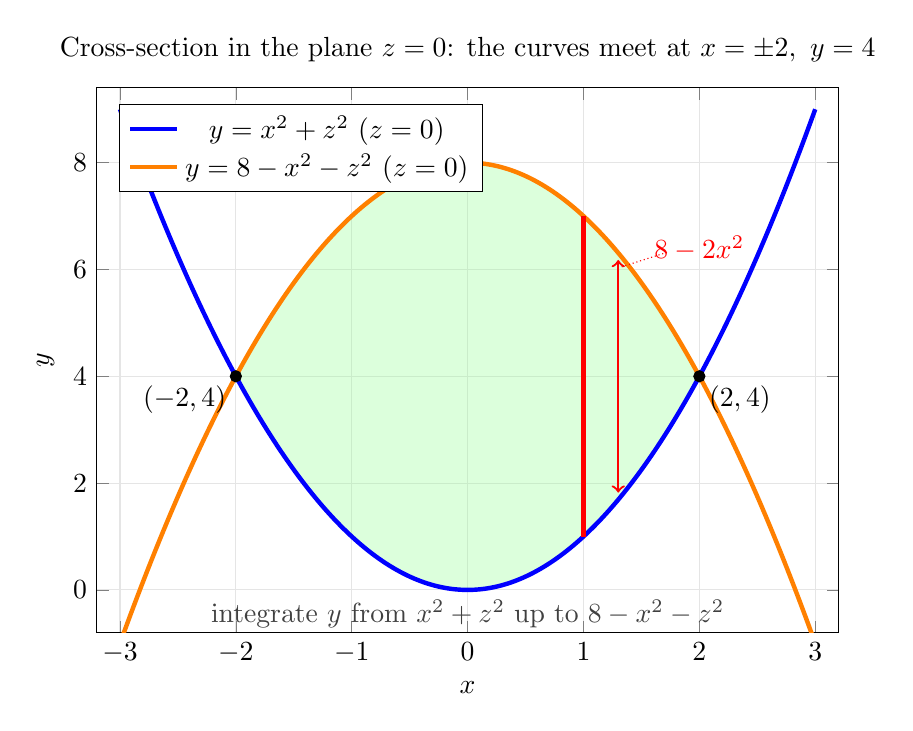
\begin{tikzpicture}
\begin{axis}[
    width=11cm, height=8.5cm,
    xlabel=$x$, ylabel=$y$,
    xmin=-3.2, xmax=3.2, ymin=-0.8, ymax=9.4,
    title={Cross-section in the plane $z=0$: the curves meet at $x=\pm2,\ y=4$},
    legend pos=north west,
    grid=major, grid style={black!10},
]
% invisible helper paths restricted to the overlap region |x| <= 2
\addplot[draw=none, domain=-2:2, samples=100, name path=L, forget plot] {x^2};
\addplot[draw=none, domain=-2:2, samples=100, name path=U, forget plot] {8-x^2};
% shaded lens = the solid seen edge-on
\addplot[green!45, opacity=0.30, draw=none, forget plot] fill between[of=U and L];
% the two parabolas
\addplot[blue, ultra thick, domain=-3:3, samples=200] {x^2};
\addlegendentry{$y=x^2+z^2\ (z=0)$}
\addplot[orange, ultra thick, domain=-3:3, samples=200] {8-x^2};
\addlegendentry{$y=8-x^2-z^2\ (z=0)$}
% intersection points
\addplot[only marks, mark=*, mark size=2, black, forget plot] coordinates {(-2,4) (2,4)};
\node[below left] at (axis cs:-2,4) {$(-2,4)$};
\node[below right] at (axis cs:2,4) {$(2,4)$};
% a typical vertical strip = the limits of the innermost integral
\addplot[red, ultra thick, forget plot] coordinates {(1,1) (1,7)};
\draw[<->, red, thick] (axis cs:1.3,1.8225) -- (axis cs:1.3,6.1775);
\node[red] at (axis cs:2.0,6.4) {$8-2x^2$};
\draw[red, thin, densely dotted] (axis cs:1.72,6.32) -- (axis cs:1.33,6.05);
\node[black!75] at (axis cs:0,-0.45)
     {integrate $y$ from $x^2+z^2$ up to $8-x^2-z^2$};
\end{axis}
\end{tikzpicture}
\end{document}
